%%%%%%%%%%%%%%%%%%%%%%%%%%%%%%%%%%%%%%%%%
% Masters/Doctoral Thesis 
% LaTeX Template
% Version 2.5 (27/8/17)
%
% This template was downloaded from:
% http://www.LaTeXTemplates.com
%
% Version 2.x major modifications by:
% Vel (vel@latextemplates.com)
%
% This template is based on a template by:
% Steve Gunn (http://users.ecs.soton.ac.uk/srg/softwaretools/document/templates/)
% Sunil Patel (http://www.sunilpatel.co.uk/thesis-template/)
%
% Template license:
% CC BY-NC-SA 3.0 (http://creativecommons.org/licenses/by-nc-sa/3.0/)
%
%%%%%%%%%%%%%%%%%%%%%%%%%%%%%%%%%%%%%%%%%

%----------------------------------------------------------------------------------------
%	PACKAGES AND OTHER DOCUMENT CONFIGURATIONS
%----------------------------------------------------------------------------------------
\PassOptionsToPackage{russian,english}{babel}
\documentclass[
12pt, % The default document font size, options: 10pt, 11pt, 12pt
oneside, % Two side (alternating margins) for binding by default, uncomment to switch to one side
english, % ngerman for German,
singlespacing, % Single line spacing, alternatives: onehalfspacing or doublespacing
%draft, % Uncomment to enable draft mode (no pictures, no links, overfull hboxes indicated)
%nolistspacing, % If the document is onehalfspacing or doublespacing, uncomment this to set spacing in lists to single
%liststotoc, % Uncomment to add the list of figures/tables/etc to the table of contents
%toctotoc, % Uncomment to add the main table of contents to the table of contents
%parskip, % Uncomment to add space between paragraphs
%nohyperref, % Uncomment to not load the hyperref package
headsepline, % Uncomment to get a line under the header
%chapterinoneline, % Uncomment to place the chapter title next to the number on one line
%consistentlayout, % Uncomment to change the layout of the declaration, abstract and acknowledgements pages to match the default layout
]{LabWhitepaper} % The class file specifying the document structure

% \usepackage[utf8]{inputenc} % Required for inputting international characters
% \usepackage[T1]{fontenc} % Output font encoding for international characters

% \usepackage{mathpazo} % Use the Palatino font by default
\usepackage{times}
\usepackage[T2A]{fontenc}
\usepackage[utf8]{inputenc}
\usepackage[russian,english]{babel}
\usepackage[backend=bibtex,style=authoryear,natbib=true]{biblatex} % Use the bibtex backend with the authoryear citation style (which resembles APA)
\usepackage{siunitx}
\usepackage{amsmath}
\usepackage{float}

\numberwithin{equation}{section}
\numberwithin{figure}{section}

\addbibresource{example.bib} % The filename of the bibliography

\usepackage[autostyle=true]{csquotes} % Required to generate language-dependent quotes in the bibliography

%----------------------------------------------------------------------------------------
%	MARGIN SETTINGS
%----------------------------------------------------------------------------------------

\geometry{
	paper=a4paper, % Change to letterpaper for US letter
	inner=2.5cm, % Inner margin
	outer=3.8cm, % Outer margin
	bindingoffset=.5cm, % Binding offset
	top=1.5cm, % Top margin
	bottom=1.5cm, % Bottom margin
	%showframe, % Uncomment to show how the type block is set on the page
}

%----------------------------------------------------------------------------------------
%	THESIS INFORMATION
%----------------------------------------------------------------------------------------

\thesistitle{Моделирование эжектируемого потока} % Your thesis title, this is used in the title and abstract, print it elsewhere with \ttitle
% \supervisor{Dr. James \textsc{Smith}} % Your supervisor's name, this is used in the title page, print it elsewhere with \supname
\examiner{Маштаков А.П.} % Your examiner's name, this is not currently used anywhere in the template, print it elsewhere with \examname
\degree{Студент} % Your degree name, this is used in the title page and abstract, print it elsewhere with \degreename
\student{Готовцев А.Г А4М6102} % Your name, this is used in the title page and abstract, print it elsewhere with \authorname
\addresses{} % Your address, this is not currently used anywhere in the template, print it elsewhere with \addressname

% \subject{Biological Sciences} % Your subject area, this is not currently used anywhere in the template, print it elsewhere with \subjectname
\keywords{} % Keywords for your thesis, this is not currently used anywhere in the template, print it elsewhere with \keywordnames
\university{{Балтийский государственный технический универсистет "Военмех" им. Д.Ф. Устинова}} % Your university's name and URL, this is used in the title page and abstract, print it elsewhere with \univname
\department{{Факультет А "Ракетно-космической техники"}} % Your department's name and URL, this is used in the title page and abstract, print it elsewhere with \deptname
\group{{Кафедра А4 «Стартовые и технические комплексы ракет и космических аппаратов»}} % Your research group's name and URL, this is used in the title page, print it elsewhere with \groupname
% \faculty{{Faculty Name}} % Your faculty's name and URL, this is used in the title page and abstract, print it elsewhere with \facname

\AtBeginDocument{
\hypersetup{pdftitle=\ttitle} % Set the PDF's title to your title
\hypersetup{pdfauthor=\studentname} % Set the PDF's author to your name
\hypersetup{pdfkeywords=\keywordnames} % Set the PDF's keywords to your keywords
\hypersetup{hidelinks}
}

\sisetup{per-mode = fraction, fraction-function=\dfrac}
\DeclareSIUnit\pascal{Па}
\DeclareSIUnit\metre{м}
\DeclareSIUnit\second{c}

\begin{document}

\frontmatter % Use roman page numbering style (i, ii, iii, iv...) for the pre-content pages

\pagestyle{plain} % Default to the plain heading style until the thesis style is called for the body content

%----------------------------------------------------------------------------------------
%	TITLE PAGE
%----------------------------------------------------------------------------------------

\begin{titlepage}
	\begin{center}

		% \vspace*{.06\textheight}
		{\Large \univname\par}
		\vspace{0.4cm} % University name
		{\large \deptname\par}
		\vspace{0.2cm}
		{\large \groupname\par}
		\vspace{0.4cm} % Research group name and department name
		\begin{figure}[h]
			\centering
			
\includegraphics[scale=0.15]{Figures/UniversityLogoLarge.png}
		\end{figure}
		\vspace{2cm}
		{\Large Расчетно-графическая работа\par} % Thesis type
		\vspace{0.5cm}
		{\huge \bfseries \ttitle\par}
		\vspace{4cm} % Thesis title
		\begin{minipage}[t]{1\textwidth}
			\begin{flushright} \large
				\emph{Студент:}\\
				{\studentname} \\% Author name - remove the \href bracket to remove the link
				\emph{Преподаватель:} \\
				{\examname}
			\end{flushright}
		\end{minipage}\\
		\vfill
		{\large \today}% Date
	\end{center}
\end{titlepage}

%----------------------------------------------------------------------------------------
%	DECLARATION PAGE
%----------------------------------------------------------------------------------------

% \begin{declaration}
% \addchaptertocentry{\authorshipname} % Add the declaration to the table of contents
% \noindent I, \authorname, declare that this thesis titled, \enquote{\ttitle} and the work presented in it are my own. I confirm that:

% \begin{itemize} 
% \item This work was done wholly or mainly while in candidature for a research degree at this University.
% \item Where any part of this thesis has previously been submitted for a degree or any other qualification at this University or any other institution, this has been clearly stated.
% \item Where I have consulted the published work of others, this is always clearly attributed.
% \item Where I have quoted from the work of others, the source is always given. With the exception of such quotations, this thesis is entirely my own work.
% \item I have acknowledged all main sources of help.
% \item Where the thesis is based on work done by myself jointly with others, I have made clear exactly what was done by others and what I have contributed myself.\\
% \end{itemize}

% \noindent Signed:\\
% \rule[0.5em]{25em}{0.5pt} % This prints a line for the signature

% \noindent Date:\\
% \rule[0.5em]{25em}{0.5pt} % This prints a line to write the date
% \end{declaration}

% \cleardoublepage

%----------------------------------------------------------------------------------------
%	QUOTATION PAGE
%----------------------------------------------------------------------------------------

% \vspace*{0.2\textheight}

% \noindent\enquote{\itshape Thanks to my solid academic training, today I can write hundreds of words on virtually any topic without possessing a shred of information, which is how I got a good job in journalism.}\bigbreak

% \hfill Dave Barry

%----------------------------------------------------------------------------------------
%	ABSTRACT PAGE
%----------------------------------------------------------------------------------------

% \begin{abstract}
% \addchaptertocentry{\abstractname} % Add the abstract to the table of contents
% The Thesis Abstract is written here (and usually kept to just this page). The page is kept centered vertically so can expand into the blank space above the title too\ldots
% \end{abstract}

%----------------------------------------------------------------------------------------
%	ACKNOWLEDGEMENTS
%----------------------------------------------------------------------------------------

% \begin{acknowledgements}
% \addchaptertocentry{\acknowledgementname} % Add the acknowledgements to the table of contents
% The acknowledgments and the people to thank go here, don't forget to include your project advisor\ldots
% \end{acknowledgements}

%----------------------------------------------------------------------------------------
%	LIST OF CONTENTS/FIGURES/TABLES PAGES
%----------------------------------------------------------------------------------------

\tableofcontents % Prints the main table of contents

% \listoffigures % Prints the list of figures

% \listoftables % Prints the list of tables

%----------------------------------------------------------------------------------------
%	ABBREVIATIONS
%----------------------------------------------------------------------------------------

% \begin{abbreviations}{ll} % Include a list of abbreviations (a table of two columns)

% \textbf{LAH} & \textbf{L}ist \textbf{A}bbreviations \textbf{H}ere\\
% \textbf{WSF} & \textbf{W}hat (it) \textbf{S}tands \textbf{F}or\\

% \end{abbreviations}

%----------------------------------------------------------------------------------------
%	PHYSICAL CONSTANTS/OTHER DEFINITIONS
%----------------------------------------------------------------------------------------

% \begin{constants}{lr@{${}={}$}l} % The list of physical constants is a three column table

% % The \SI{}{} command is provided by the siunitx package, see its documentation for instructions on how to use it

% Speed of Light & $c_{0}$ & \SI{2.99792458e8}{\meter\per\second} (exact)\\
% %Constant Name & $Symbol$ & $Constant Value$ with units\\

% \end{constants}

%----------------------------------------------------------------------------------------
%	SYMBOLS
%----------------------------------------------------------------------------------------

\begin{symbols}{lll} % Include a list of Symbols (a three column table)

$P_\text{п}$ & давление в приструйной зоне, &	\si{\text{Па}} \\
$P_\text{в}$ & внешнее давление, & \si{\text{Па}} \\
$h_\text{э}$ & потери давления на эжекцию воздуха, & \si{\text{Па}} \\
$h_\text{м}$ & потери давления на местных сопротивлениях, & \si{\text{Па}} \\
$\upsilon_\text{э}$	& скорость эжектируемого воздуха & \si[per-mode = fraction]{\text{м}\per\second} \\
$\rho$ & плотность воздуха & \si{\text{кг}\per\text{м}\cubed}\\
$h_\text{с}$ & потери давления при сужении канала & \si{\text{Па}} \\
$h_\text{р}$ & потери давления при расширении канала & \si{\text{Па}} \\
$h_\text{п}$ & потери давления при повороте канала & \si{\text{Па}} \\
$C_\text{ст}$ & эжекционная способность струи & \si[per-mode = fraction]{\text{м}\squared\per\second} \\
$r_\text{ст}$ & радиус границы струи & \si{\text{м}} \\
$m$ & расход газа & \si{\text{м}\cubed\per\second} \\
$Q_\text{зв}$ & расход газа в звуковом сечении & \si{\text{м}\cubed\per\second} \\
$x_\text{зв}$ & осевая координата звукового сечения \si{\text{м}} & \\
$l$ & скорость газа в звуковом сечении & \si{\text{м}\per\second} \\
$\varphi$ & коэффициент потерь в сопле Лаваля 1 & \\
$F_\text{кр}$ & площадь критического сечения сопла & \si{\text{м}\squared} \\
$F_\text{a}$ & площадь выходного сечения сопла & \si{\text{м}\squared} \\
$B$ & коэффициент потерь в сопле Лаваля 2 & \\
$P_{0}$ & начальное давление в камере сгорания & \si{\text{Па}} \\
$P_\text{а}$ & давление в выходном сечении сопла & \si{\text{Па}} \\
$R$ & универсальная газовая постоянная & \si[per-mode = fraction]{\text{Дж}\per(\text{моль}.\text{К})} \\
$T$ & абсолютная температура торможения & \si{\text{К}} \\
$\varGamma$ & показатель адиабаты & \\
$M$ & число Маха & \\
$\eta$ & ??? & \\
% $P$ & power & \si{\watt} (\si{\joule\per\second}) \\
%Symbol & Name & Unit \\

% \addlinespace % Gap to separate the Roman symbols from the Greek

% $\omega$ & angular frequency & \si{\radian} \\

\end{symbols}

%----------------------------------------------------------------------------------------
%	DEDICATION
%----------------------------------------------------------------------------------------

% \dedicatory{For/Dedicated to/To my\ldots} 

%----------------------------------------------------------------------------------------
%	THESIS CONTENT - CHAPTERS
%----------------------------------------------------------------------------------------

\mainmatter % Begin numeric (1,2,3...) page numbering

\pagestyle{thesis} % Return the page headers back to the "thesis" style

% Include the chapters of the thesis as separate files from the Chapters folder
% Uncomment the lines as you write the chapters

\chapter{Введение}

В работе рассматривается процесс эжекции воздуха из прилегающей к сверхзвуковой струе среды. Процесс истечения происходит в камеру ограниченного диаметра. В качестве результата работы необходимо определить изменение давления в приструйной зоне. При расчете необходимо учесть потери давления на эжекцию воздуха и потери на местные споротивления в эжектируемом потоке, затекающем внутрь камеры.
\chapter{Расчетная модель}
\label{Chapter2}
\setlength{\parindent}{0pt}

\section{Описание}
Для расчета изменений давления в приструйной зоне во времени примем расчетный цикл. На каждой его итерации будем рассчитывать величину потерь на эжекцию воздуха и вычитать её из текущего значения давления. Тем самым будет получено новое значение давления в приструйной зоне, которое будет использовано в следующей итерации как текущее. Изменящееся внешние давление будет оказывать влияние на режим истечения струи и её эжектирующую способность, что также повлечет за собой изменение величины потерь.

\section{Основные соотношения}
Основным расчетным соотношением является формула 

\begin{equation}
    \label{eqn:MainPressure}
    P_\text{п}=P_\text{в}-h_\text{э}-h_\text{м},
\end{equation}

в которой отражены потери полного давления на эжекцию воздуха и потери давления на местных сопротивлениях. Полное давление приравнено к окружающему. Потери на эжекцию определяеются следующим соотношением

\begin{equation}
    \label{eqn:EjectionLosses}
    h_\text{э}=\dfrac{\rho\upsilon_\text{э}^2}{2}.
\end{equation}

Потери на потери давления на местных сопротивлениях определяются в соответствие с расчетной схемой, изображенной на \hyperref[fig:LossesScheme]{рисунке 2.2.1}

\begin{figure}[H]
    \label{fig:LossesScheme}
    \centering
    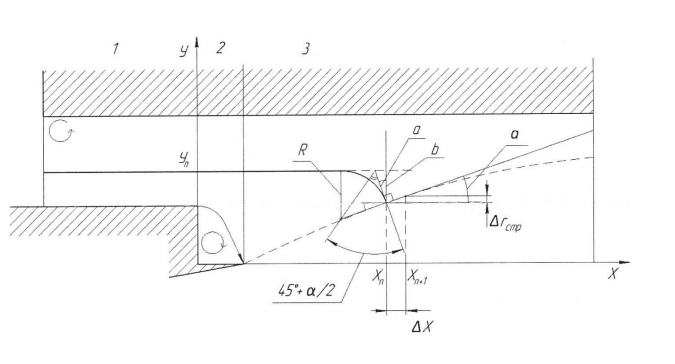
\includegraphics[height=6cm]{Figures/Scheme.png}
    \caption{Схема расчета потерь на местных споротивлениях}
\end{figure}

По схеме, эти потери выражаются в трех составляющих - потерях на внезапное сужение канала, на участке 1, потерях на внезапное расширение канала, на участке 2, и поворот канала, на участке 3. Соответственно, имеем формулу

\begin{equation}
    \label{eqn:LocalLosses}
    h_\text{м}=h_\text{с}+h_\text{р}+h_\text{п}.
\end{equation}

Таким образом, имея ввиду расчетные соотношения \hyperref[eqn:EjectionLosses]{2.2.2}, \hyperref[eqn:LocalLosses]{2.2.3}, требуется определить зависимости потерь от параметров течения струи.

\section{Потери на эжекцию}
В соответствии с \hyperref[eqn:EjectionLosses]{формулой 2.2.2} для определения потерь на эжектирующем участке струи необходимо определить скорость эжектируемого потока для каждого сечения. Для этого воспользуемся соотношением

\begin{equation}
    \label{eqn:EjectionVelocity}
    \upsilon_\text{э}=\dfrac{C_\text{ст}}{2\pi\rho r_\text{ст}}.
\end{equation}

Величина $C_\text{ст}$ - эжекционная способность струи, принимается постоянной по её длине. Для определения введем формулу

\begin{equation}
    \label{eqn:EjectionAbility}
    C_\text{ст}=\dfrac{Q_\text{зв}-m}{x_\text{зв}}.
\end{equation}

Формула для расхода

\begin{equation}
    \label{eqn:Consumption}
    m=\varphi(\dfrac{F_\text{кр}BP_{0}}{\sqrt{RT}}),
\end{equation}

где $F_\text{кр}$ - площадь критического сечения сопла, определяемая как

\begin{equation}
    \label{eqn:CriticalSquare}
    F_\text{кр}=\dfrac{F_\text{а}}{\dfrac{1}{M^2}((\dfrac{2}{\gamma+1})(1+M^2 \dfrac{\gamma-1}{2}))^{\dfrac{\gamma+1}{\gamma-1}}},
\end{equation}

a также $B$ и $\varphi$, коэффициенты потерь в сопле Лаваля,

\begin{equation}
    \label{eqn:LavalKoef2}
    B=(\dfrac{2}{\gamma+1})^{\dfrac{\gamma+1}{2(\gamma-1)}},
\end{equation}

\begin{equation}
    \label{eqn:LavalKoef1}
    \varphi=0.98,
\end{equation}

и начальное давление в камере сгорания

\begin{equation}
    \label{eqn:StartPressure}
    P_\text{0}=P_\text{а}(1+\dfrac{\gamma-1}{2} M^2)^{\dfrac{\gamma}{\gamma-1}}.
\end{equation}

Величины $Q_\text{зв}$ и $x_\text{зв}$ характеризуют звуковое сечение - такое, в котором скорость истечения газа равно скорости звука. Сначала определяется координата сечения на оси струи

\begin{equation}
    \label{eqn:SoundCoord}
    x_\text{зв}=(13.28 \sqrt{\gamma M^2} + 11.8) \sqrt[3]{\eta}-23.57.
\end{equation}

Затем, по данным рассчета геометрии струи определяется радиус этого сечения. С его помощью определяем расход через звуковое сечение

\begin{equation}
    \label{eqn:SoundConsumption}
    Q_\text{зв}=0.217 \pi l r_\text{ст}^2,
\end{equation}

где, соответственно

\begin{equation}
    \label{eqn:SoundVelocity}
    l=\sqrt{\dfrac{\gamma}{RT}} P_\text{в} \sqrt{\dfrac{\gamma+1}{2}}.
\end{equation}

Таким образом, имеем все необходимые соотношения для определения величины потерь на эжекцию воздуха по \hyperref[eqn:EjectionLosses]{формуле 2.2.2}.

\section{Потери на местных сопротивлениях}
Из \hyperref[eqn:LocalLosses]{формулы местных потерь 2.2.3} имеем потери при внезапном сужении канала, выраженные формулой

\begin{equation}
    \label{eqn:ConstrictionLosses}
    h_\text{с}=\zeta_\text{с} \dfrac{\upsilon_{12}^2}{2g},
\end{equation}

потери при внезапном расширении канала, выраженные формулой

\begin{equation}
    \label{eqn:ExpansionLosses}
    h_\text{рв}=\zeta_\text{р} \dfrac{\upsilon_{23}^2}{2g},
\end{equation}

и, потери при повороте, выраженные формулой

\begin{equation}
    \label{eqn:RotationLosses}
    h_\text{рв}=\zeta_\text{п} \dfrac{\upsilon_{23\text{ср}}^2}{2g}.
\end{equation}

Коэффициент потерь при внезапном сужении постоянен и равен

\begin{equation}
    \label{eqn:ConstrictionLossesCoef}
    \zeta_\text{с} = 0.5
\end{equation}

потерь при внезапном расширении определяется перепадом сечений и равен

\begin{equation}
    \label{eqn:ExpansionLossesCoef}
    \zeta_\text{р}=(1-\dfrac{S_{2}}{S_{3}})^2.
\end{equation}

Коэффициент потерь при повороте канала определяется углом поворота

\begin{equation}
    \label{eqn:RotationLossesCoef}
    \zeta_\text{п}=0.95 (\sin(\dfrac{\alpha}{2}))^2 + 2.05(\sin(\dfrac{\alpha}{2}))^4.
\end{equation}

Скорости газа во всех случаях определяются из закона постоянства расхода.


\chapter{Результаты расчета}
\label{Chapter3}
\setlength{\parindent}{0pt}

\section{Исходные данные}
$P_\text{в}=10^5$ \si{\text{Па}} - внешнее давление в начальный момент времени \\
$\rho=1.2041$ \si{\text{кг}\per\text{м}\cubed} - плотность воздуха \\
$F_\text{a}=0.5$ \si{\text{м}\squared} - площадь выходного сечения сопла \\
$P_\text{а}=0.8\cdot 10^5$ \si{\text{Па}} - давление в выходном сечении сопла в начальный момент времени \\
$R=287$\si[per-mode = fraction]{\text{Дж}\per(\text{моль}.\text{К})} - универсальная газовая постоянная \\
$T=293$ \si{\text{К}} - температура торможения \\
$\varGamma=1.4$ - показатель адиабаты \\
$M=3$ - число Маха \\
$d_\text{а}=0.8$ \si{\text{м}} - диаметр выходного сечения сопла \\
$d_\text{к}=1$ \si{\text{м}} - диаметр кормы \\
$d_\text{тр}=1.2$ \si{\text{м}} - диаметр трубы \\
$\alpha=10$ \si{\degree} - угол полураствора сопла \\
$x=10$ \si{\text{м}} - длина эжектирующего участка \\

\section{Изменения основных величин}

\begin{figure}[H]
    \label{fig:ExternalPressure}
    \centering
    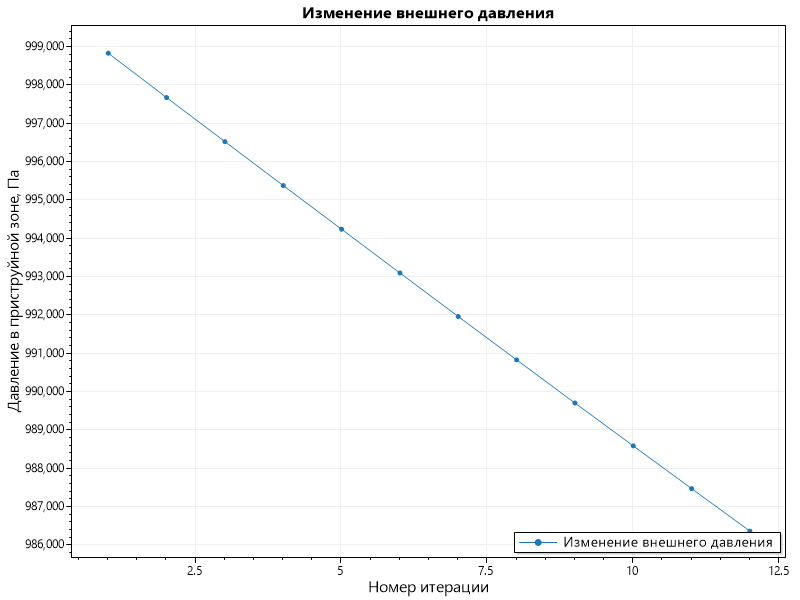
\includegraphics[width=13cm]{Figures/Pext.png}
    \caption{Изменение давления в приструйной зоне}
\end{figure}

\begin{figure}[H]
    \label{fig:EjectionLosses}
    \centering
    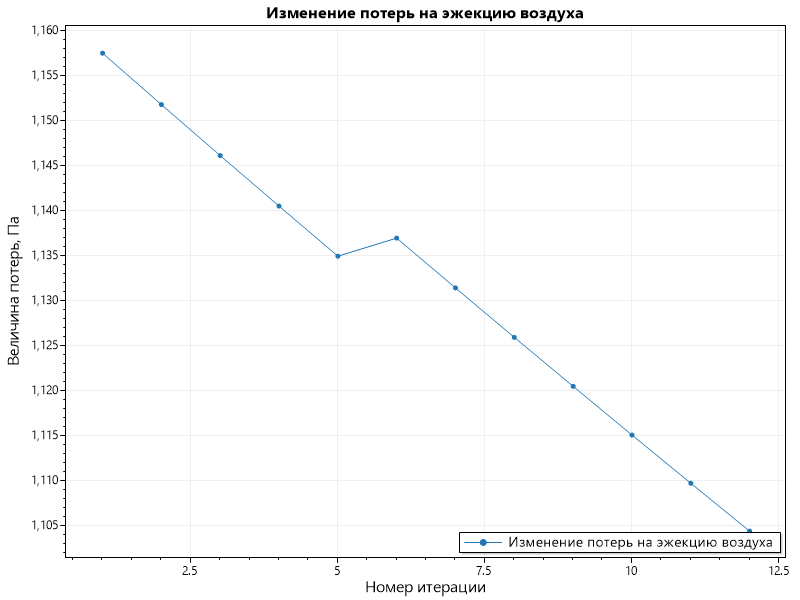
\includegraphics[width=13cm]{Figures/Hej.png}
    \caption{Изменение потерь на эжекцию приструйсного воздуха}
\end{figure}

\begin{figure}[H]
    \label{fig:LocalLosses}
    \centering
    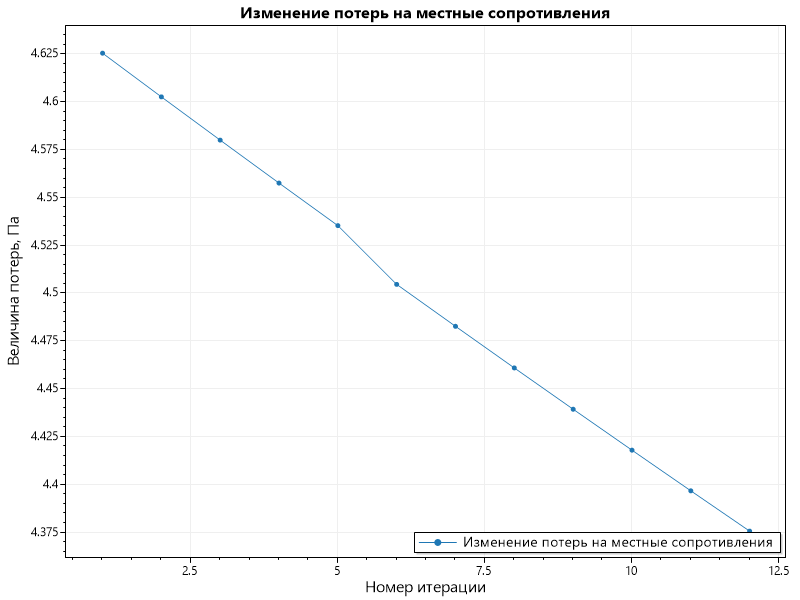
\includegraphics[width=13cm]{Figures/Hl.png}
    \caption{Изменение потерь на местных сопротивлениях в зазоре}
\end{figure}

\begin{figure}[H]
    \label{fig:FluidStructure}
    \centering
    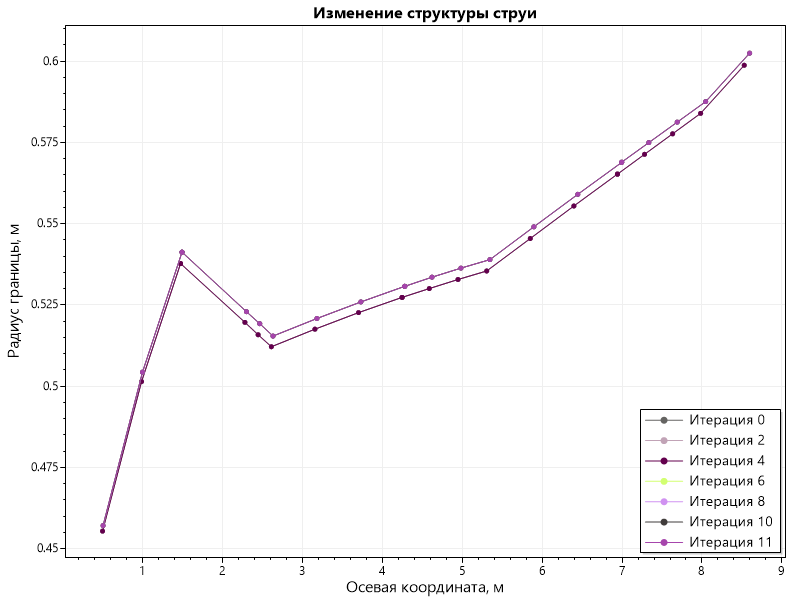
\includegraphics[width=13cm]{Figures/FluidStruct.png}
    \caption{Изменение структуры струи}
\end{figure}

\chapter{Заключение}

В процессе выполнения работы по представленной математической модели был выполнен итерационный расчет. На каждой итерации производился расчет геометрии струи, скорости эжектируемого воздуха и потерь. Изменения внешнего давления в приструйной зоне, возникающие в следствие эжекции, учитывались при каждой последующей итерации расчета. В момент, когда границы струи достигли стенок камеры (6 итерация), была также пересчитана площадь эжектирующего участка. После этого, было произведено еще 6 итераций.

В результате выполнения расчета выявлены зависимости, представленные графически в \hyperref[Chapter3]{главе 3}. Из них видно, что давление в приструйной зоне линейно падает \hyperref[fig:ExternalPressure]{(рис. 3.2.1)} в пределах от 998,2 кПа до 986,4 кПа. Данное обстоятельство приводит к расширению границ струи в среднем на 0.005 м по всех длине \hyperref[fig:FluidStructure]{(рис. 3.2.4)} и последующему их пересечению со стенками камеры.
%\include{Chapters/Chapter5} 

%----------------------------------------------------------------------------------------
%	THESIS CONTENT - APPENDICES
%----------------------------------------------------------------------------------------

% \appendix % Cue to tell LaTeX that the following "chapters" are Appendices

% Include the appendices of the thesis as separate files from the Appendices folder
% Uncomment the lines as you write the Appendices

% % Appendix A

\chapter{Frequently Asked Questions} % Main appendix title

\label{AppendixA} % For referencing this appendix elsewhere, use \ref{AppendixA}

\section{How do I change the colors of links?}

The color of links can be changed to your liking using:

{\small\verb!\hypersetup{urlcolor=red}!}, or

{\small\verb!\hypersetup{citecolor=green}!}, or

{\small\verb!\hypersetup{allcolor=blue}!}.

\noindent If you want to completely hide the links, you can use:

{\small\verb!\hypersetup{allcolors=.}!}, or even better: 

{\small\verb!\hypersetup{hidelinks}!}.

\noindent If you want to have obvious links in the PDF but not the printed text, use:

{\small\verb!\hypersetup{colorlinks=false}!}.

%\include{Appendices/AppendixB}
%\include{Appendices/AppendixC}

%----------------------------------------------------------------------------------------
%	BIBLIOGRAPHY
%----------------------------------------------------------------------------------------

% \printbibliography[heading=bibintoc]

%----------------------------------------------------------------------------------------

\end{document}
